\documentclass[runningheads]{llncs}
\usepackage{graphicx}

\usepackage{hyperref} % For clickable \href{} URLs

%Code:
\usepackage{listings}
\usepackage{color}
\usepackage{cite}
\usepackage{amsmath,amssymb,amsfonts}
\usepackage{graphicx}
\usepackage{caption}
\usepackage{subcaption}
\usepackage{textcomp}
\usepackage{xcolor}
\usepackage{dirtree} % Tree diagram
\usepackage{mathtools} % Pseudocode packages:
\usepackage{algorithm}
\usepackage{algorithmic}
\usepackage{amssymb}
%\usepackage{refcheck}
\usepackage{breqn} % For dmath, multiline math

\definecolor{dkgreen}{rgb}{0,0.6,0}
\definecolor{gray}{rgb}{0.5,0.5,0.5}
\definecolor{mauve}{rgb}{0.58,0,0.82}
\lstset{frame=tb,
  language=Java,
  aboveskip=3mm,
  belowskip=3mm,
  showstringspaces=false,
  columns=flexible,
  basicstyle={\small\ttfamily},
  numbers=none,
  numberstyle=\tiny\color{gray},
  keywordstyle=\color{blue},
  commentstyle=\color{dkgreen},
  stringstyle=\color{mauve},
  breaklines=true,
  breakatwhitespace=true,
  tabsize=3
}

\newcommand{\blue}[1]{\noindent{\textcolor{blue}{\textbf{#1}}}}

%\newcommand{\sw}[1]{\textbf{\textcolor{red}{SW: #1}}}

\begin{document}

\title{CS 5220: Project Technical Report}

%\author{First Author\inst{1}\orcidID{0000-1111-2222-3333} \and
\author{Simeon Wuthier}
%
\authorrunning{F. Author et al.}

\institute{
    \textit{Department of Computer Science}\\
    \textit{University of Colorado, Colorado Springs}\\
    \email{swuthier@uccs.edu}\\
}

\maketitle
%\begin{abstract}
%Abstract
%\keywords{First keyword  \and Second keyword \and Another keyword.}
%\end{abstract}

\section{Compilation / Execute Guide}
I selected C++ as my programming language, all algorithms required for the project are fully implemented and functional. The adjustable packet drop rate percentage has been implemented in both UDP protocols on the server. After deleting the PDF on the client then re-requesting it, all three protocols return a successful transmission of the PDF file. Additional test PDFs have been included in the project files. Below are the instructions on how to execute the code files.

\subsection{Server-side}
To compile and execute part 1 (TCP), use the following code.

\begin{lstlisting}
g++ -std=c++11 TCP_Server.cpp -o TCP_Server
./TCP_Server
\end{lstlisting}

To compile and execute part 2 (UDP) with a frame loss rate of 30\% and using protocol 2 (selective repeat), use the following code. The frame loss rate can be an integer between $[0, 100]$ and the protocol must be in $[1, 2]$.

\begin{lstlisting}
g++ -std=c++11 UDP_Server.cpp -o UDP_Server -lpthread
./UDP_Server 30 2
\end{lstlisting}

\blue{Alternatively, run \emph{./run\_part1.sh} to execute part 1 (TCP),\\ and \emph{./run\_part2.sh} to execute part 2 (UDP$_1$ and UDP$_2$).}
\\
\\
The included server-side files are as follows.
\begin{itemize}
    \item \textbf{run\_part1.sh}~\textemdash~Compiles and executes \emph{TCP\_Server.cpp}.
    \item \textbf{TCP\_Server.cpp}~\textemdash~TCP basic file transfer protocol.
    \item \textbf{run\_part2.sh}~\textemdash~Compiles and executes \emph{UDP\_Server.cpp}.
    \item \textbf{UDP\_Server.cpp}~\textemdash~UDP file transfer in \emph{stop-and-wait} and \emph{selective repeat}.
\end{itemize}


\subsection{Client-side}

To compile and execute part 1 (TCP) to download \emph{SIGCOMM10-DataCenterTCP-2.pdf}, use the following code.

\begin{lstlisting}
g++ -std=c++11 TCP_Client.cpp -o TCP_Client
rm -rf SIGCOMM10-DataCenterTCP-2.pdf
./TCP_Client windom.uccs.edu SIGCOMM10-DataCenterTCP-2.pdf
\end{lstlisting}

To compile and execute part 2 (UDP) to download \emph{SIGCOMM10-DataCenterTCP-2.pdf} using protocol 2 (selective repeat), use the following code.

\begin{lstlisting}
g++ -std=c++11 UDP_Client.cpp -o UDP_Client -lpthread
rm -rf SIGCOMM10-DataCenterTCP-2.pdf
./UDP_Client windom.uccs.edu SIGCOMM10-DataCenterTCP-2.pdf 2
\end{lstlisting}

\blue{Alternatively, run \emph{./run\_part1.sh} to execute part 1, and \emph{./run\_part2.sh} to execute part 2.}
\\
\\
The included client-side files are as follows.

\begin{itemize}
    \item \textbf{run\_part1.sh}~\textemdash~Compiles and executes \emph{TCP\_Client.cpp}.
    \item \textbf{TCP\_Client.cpp}~\textemdash~TCP basic file transfer protocol.
    \item \textbf{run\_part2.sh}~\textemdash~Compiles and executes \emph{UDP\_Client.cpp}.
    \item \textbf{UDP\_Client.cpp}~\textemdash~UDP file transfer in \emph{stop-and-wait} and \emph{selective repeat}.
\end{itemize}

\begin{figure*}[htp]
\centering
\begin{subfigure}{1\linewidth}
  \centering
  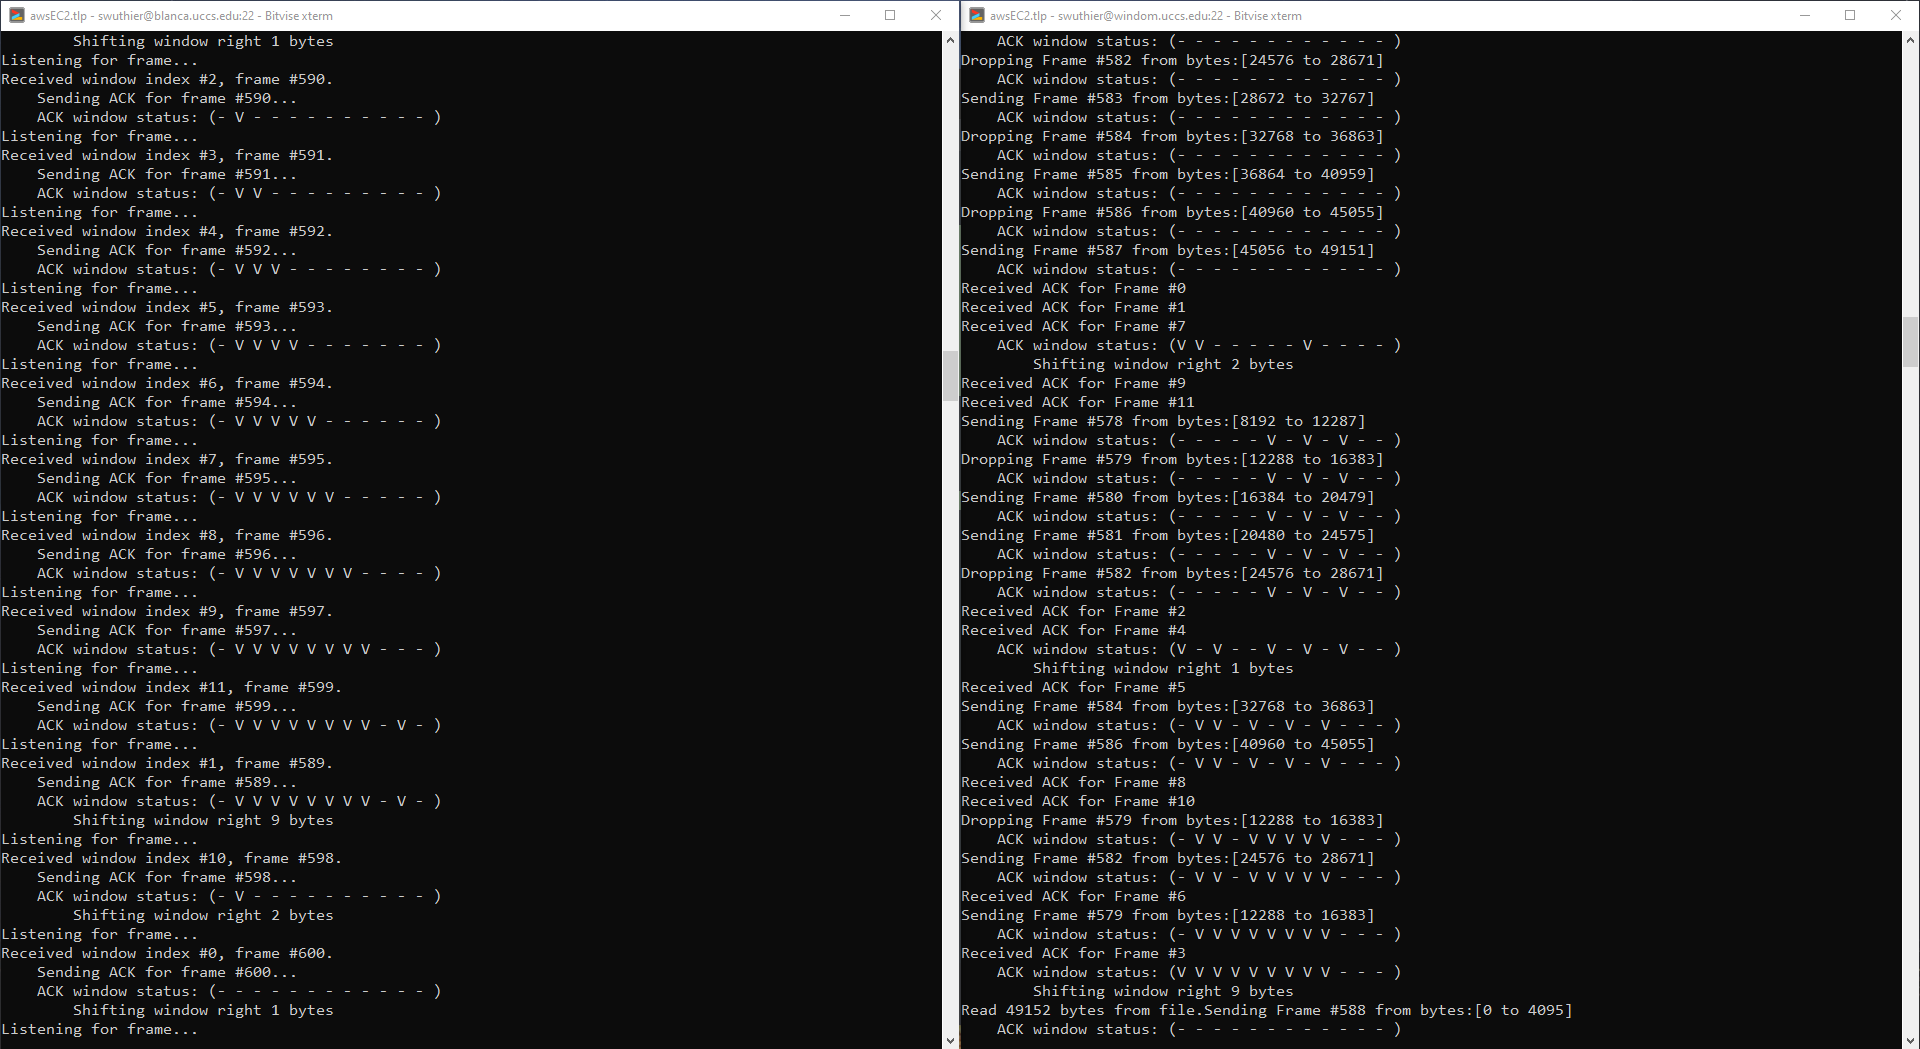
\includegraphics[width=1\linewidth]{Figures/console_drop_30.png}
  \caption{Using a drop rate of 30\% the transmissions are more non-deterministic. The left screen is the client on \emph{blanca.uccs.edu}, while the right screen is the server on \emph{windom.uccs.edu}.}
  \label{fig:console-udp1}
\end{subfigure}
%quad
\begin{subfigure}{1\linewidth}
  \centering
  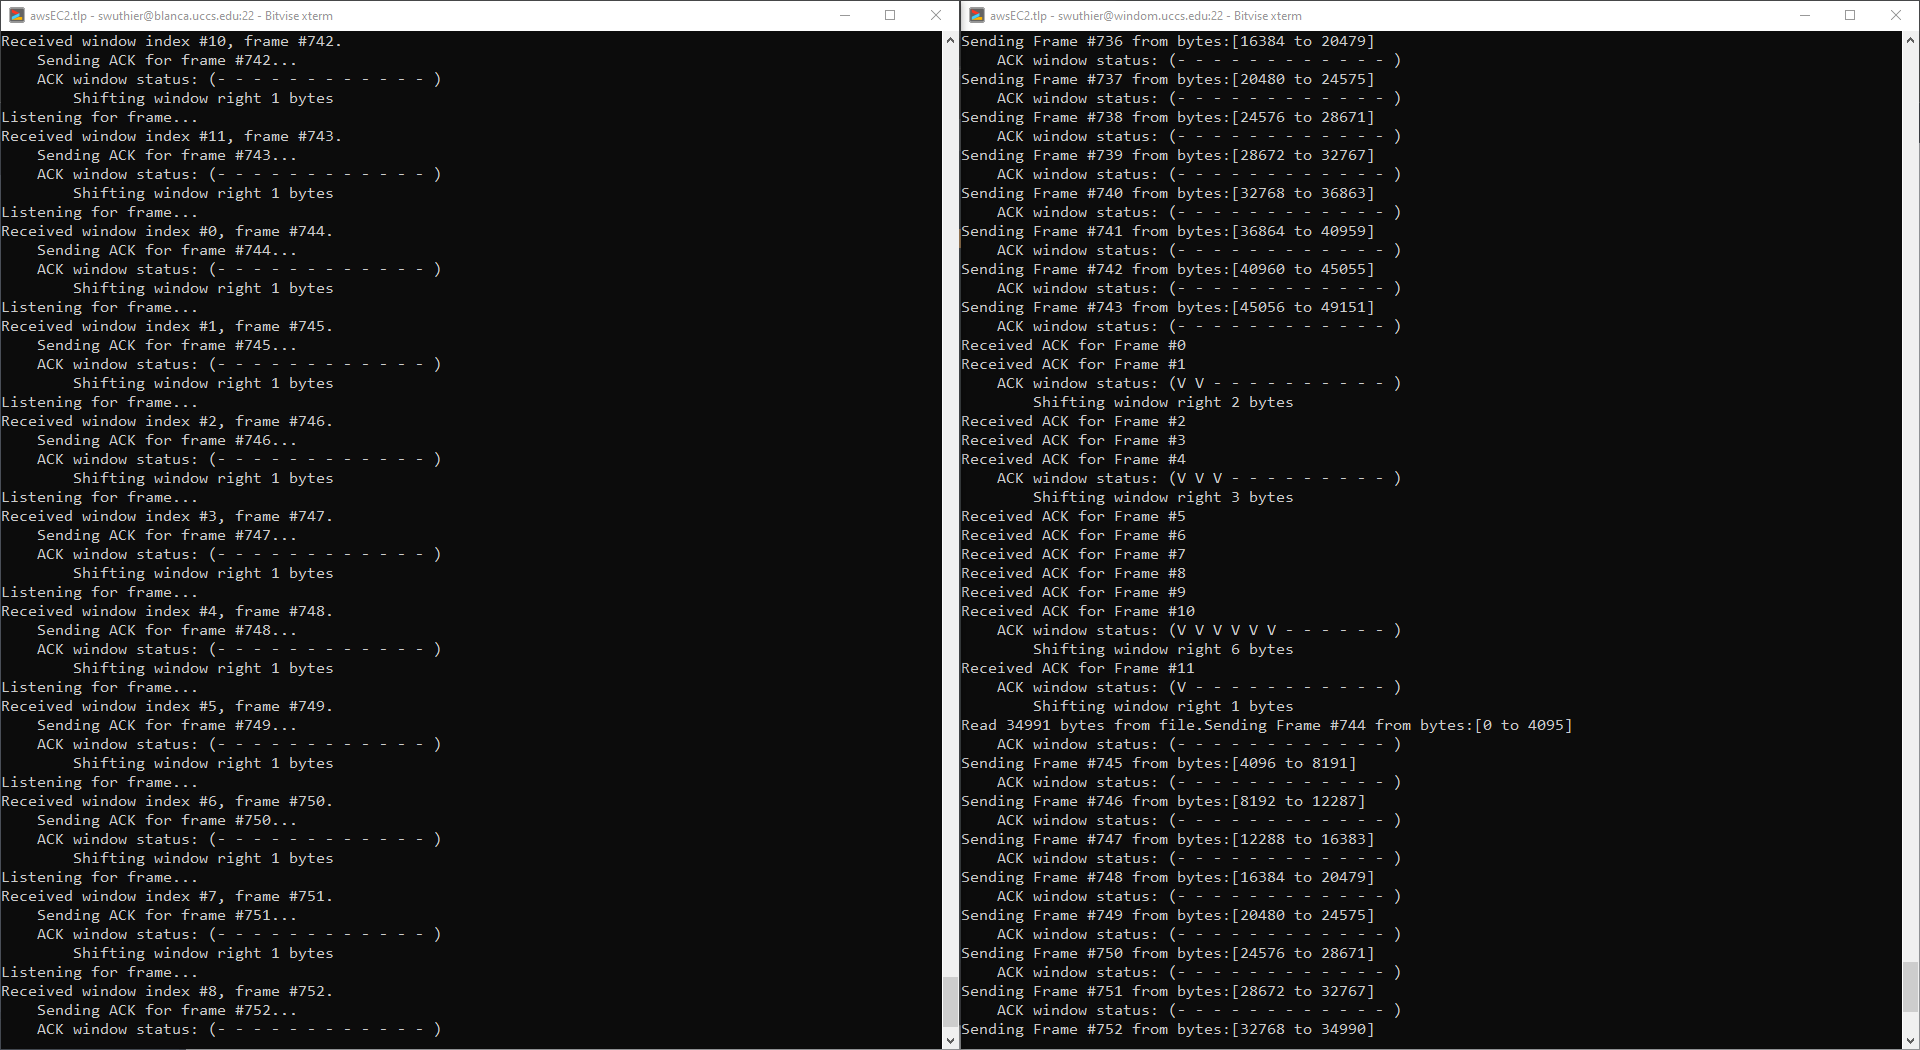
\includegraphics[width=1\linewidth]{Figures/console_drop_0.png}
  \caption{Using a drop rate of 0\% the transmissions are more uniform. The left screen is the client on \emph{blanca.uccs.edu}, while the right screen is the server on \emph{windom.uccs.edu}.}
  \label{fig:console-udp2}
\end{subfigure}
\caption{The console screen for selective repeat in UDP. For every ACK transmission the program prints the \emph{windowReceivedLog} Boolean array, where ``$-$'' means the message is pending, and ``$V$'' means the message has been received. When the window's leftmost $N$ packets are received, the window automatically shifts until the rightmost packet returns to ``$-$''. Window shifts are displayed on both the client and the server. Using \emph{blanca.uccs.edu} for the client and \emph{windom.uccs.edu} for the server, the transmissions function at maximum speed, and the PDF is readable for every protocol.\label{fig:console}}
\end{figure*}


\section{Self-testing Result}

This section discusses the verification steps for stop-and-wait and selective repeat. In both situations, the file transmits and the PDF can be opened, but the protocol-level verification requires additional steps to ensure the sliding window is properly implemented in selective repeat.
\subsection{Features / Design Comments}
The code is well-documented through comments. I implement both parts by building the framework as the baseline for the protocol. The framework includes the following functions.
\begin{itemize}
    \item \textsc{IsFrameDropped}~\textemdash~Takes a loss probability, and returns \emph{true} or \emph{false} depending on if the random number is less than the loss probability.
    \item \textsc{ComputeCrcChecksum}~\textemdash~Given a char* array and length, add all the bytes together, then take the last byte from the sum, this is the non-cryptographic hash that is used for packet payloads.
    \item \textsc{SerializeAck}~\textemdash~Creates a two-byte ack by packing the negation flag (ACK/NACK), then the sequence number.
    \item \textsc{DeserializeAck}~\textemdash~Given a char* array, extract the negation flag and sequence number.
    \item \textsc{SerializeFrame}~\textemdash~A frame consists of an end of transmission (EOT) flag, sequence number, payload size, payload, and checksum. This function packs all the data into a single char* array, ready for transmission.
    \item \textsc{DeserializeFrame}~\textemdash~Given a serialized frame, extract all data values. Returns \emph{true} if the checksum matches the cyclic redundancy check (CRC) of the frame, otherwise, it returns \emph{false} signalizing a negated ACK needs to be sent.
    \item \textsc{AsyncListenForAcksThenRespond}~\textemdash~ runs on a separate thread, and is responsible for receiving ACKs and frames, and flipping the corresponding window upon successful data transmission. Before writing to the window (\emph{WindowReceivedLog}), the program must set a mutual exclusion (mutex) lock, then unlock the data after setting the data. This is to ensure that both threads are able to maintain a single data structure at once.
    \item \textsc{Fatal}~\textemdash~Gracefully terminate the program if the socket is unable to get started, or the client is unable to connect. Once the server has started, it cannot be stopped by the client.
\end{itemize}

The server runs an infinite loop to continue accepting connections in the future, while the client terminates as soon as it receives the full file contents (denoted by the EOT flag within the frame). The flow of the protocol is split into two phases.
\begin{itemize}
    \item Phase 1: File name transmission. The client sends the file name to the server every 100ms. Upon receiving the file name on the server, the server will send an ACK if the file exists, and a NACK if the file does not exist. If the client receives a NACK then it will gracefully terminate with an ``\emph{ERROR: 404, file not found}'' error. If an ACK is received by the client, then it can proceed to the next step.
    \item Phase 2: File transmission. If the protocol is 1, then stop-and-wait will be used, otherwise, selective repeat will be used.
\end{itemize}

Selective repeat is the only protocol that utilizes \textsc{AsyncListenForAcksThenRespond}'s multi-threaded behavior. Selective repeat was programmed to be parallel because the receiver function can work alongside the more complex protocol-level code, and just update as soon as \textsc{AsyncListenForAcksThenRespond} updates \emph{WindowReceivedLog}. For the phase 1, and phase 2: stop-and-wait protocol, I use the following code to force a \emph{recvfrom} timeout, so that I can assume that a packet has been dropped, and re-send it.
\begin{lstlisting}
// Timeout after FRAMETIMEOUT milliseconds
struct timeval readTimeout;
readTimeout.tv_sec = 0;
// Convert milliseconds to microseconds
readTimeout.tv_usec = FRAMETIMEOUT * 1000;
setsockopt(sd, SOL_SOCKET, SO_RCVTIMEO, (const char*)&readTimeout, sizeof readTimeout);
\end{lstlisting}
By default, the frame timeout is 100ms. For frame timeouts of 0ms, the \emph{setsockopt} returns to the default of no timeout, where \emph{recvfrom} waits indefinitely.
The port used is 2060. For stop-and-wait, the verification is straightforward since the networking is linear, where a frame and acknowledgment alternate on both the client and server. For dropped packets, the frame is repeated when the timeout of 100ms is reached. For selective repeat, however, the logging is more verbose since the window is displayed while ACKs are received. Due to multi-threading, there is a race condition between printing the window and updating the window. On the client, there is a notification that frames are received, and an ACK/NACK is sent depending on the frame's success. On the server, there are additional messages for the window size and what byte numbers are being sent with regards to the frame number. ACKs and NACKs are displayed as well.

\subsubsection{Packet Dropping}
The following code snippet is used to determine if a packet should be dropped or not.
\begin{lstlisting}
#include <cstdlib>
// lossProbability = 0% then no frames are dropped
// lossProbability = 100% then all frames are dropped
bool isFrameDropped(int lossProbability) {
    int r = 1 + rand() % 100; // 1 to 100
    return r <= lossProbability;
}
\end{lstlisting}
If \textsc{IsFrameDropped(X)} returns \emph{true}, then the server will withhold the \emph{sendto} function from being called. This is included in selective repeat \emph{and} stop-and-wait.

\subsection{Trace of Flow Control for Lost Frames}
\begin{figure*}[htp]
\centering
\begin{subfigure}{0.32\linewidth}
  \centering
  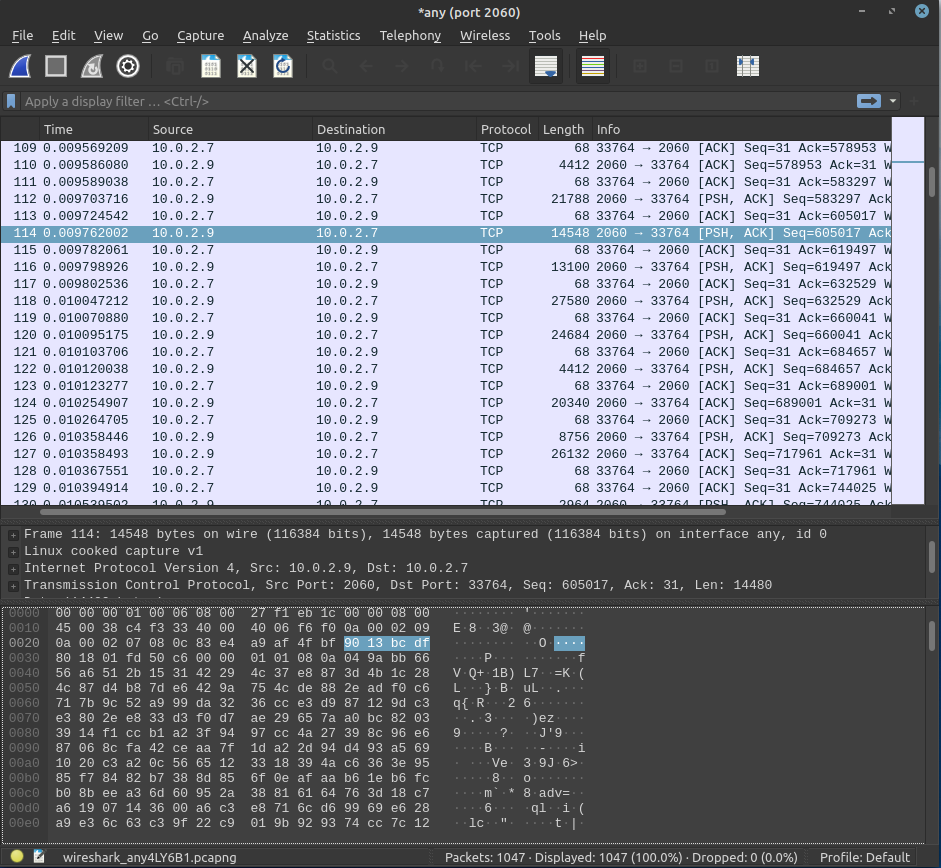
\includegraphics[width=1\linewidth]{Figures/TCP_packet_capture.png}
 stop-and-wait as well as  \caption{TCP file transfer using the classical protocol.\vspace{55pt}}
  \label{fig:tcp}
\end{subfigure}
\begin{subfigure}{0.32\linewidth}
  \centering
  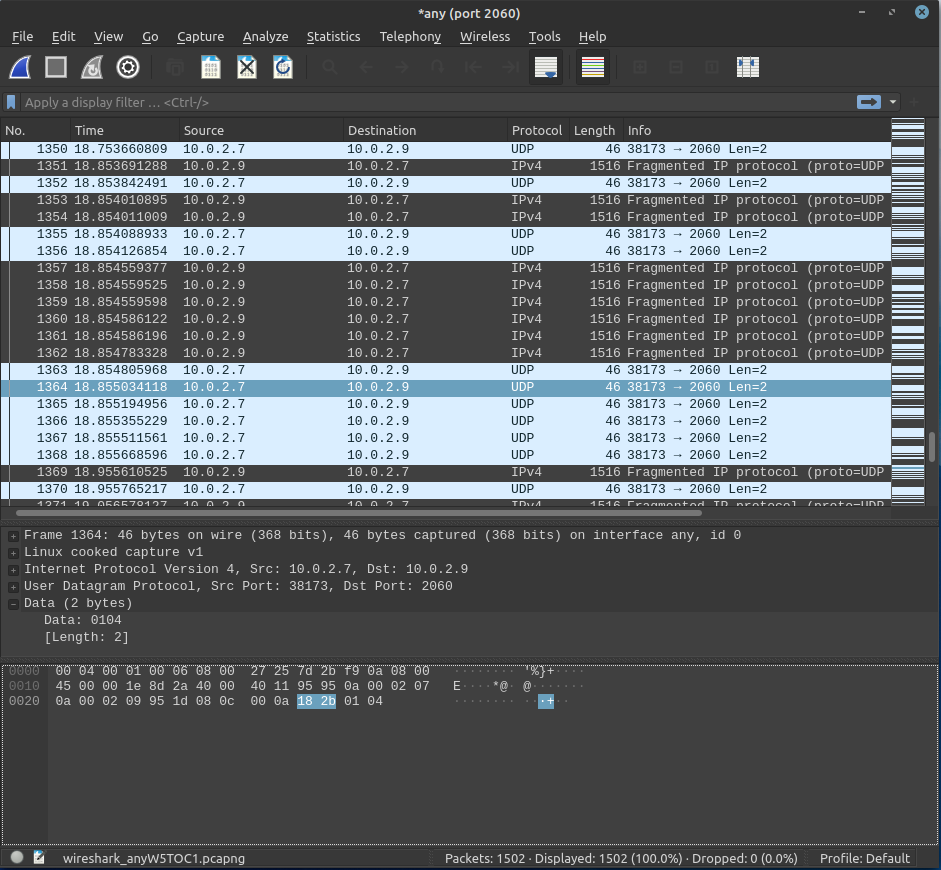
\includegraphics[width=1\linewidth]{Figures/UDP2_packet_capture.png}
  \caption{UDP selective repeat file transfer using a window size of 10 and a packet drop rate of 30\%. There is a greater variation because dropped traffic causes NACK transmissions.}
  \label{fig:udp2}
\end{subfigure}
\begin{subfigure}{0.32\linewidth}
  \centering
  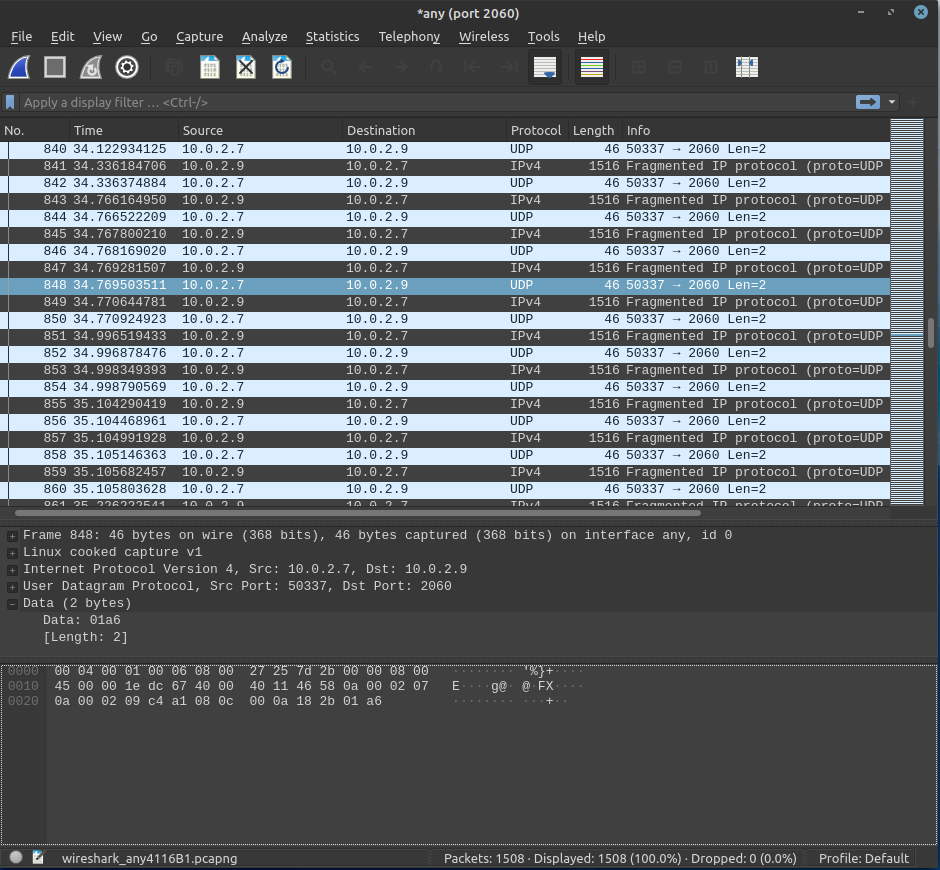
\includegraphics[width=1\linewidth]{Figures/UDP1_packet_capture.png}
  \caption{UDP stop-and-wait file transfer using a packet drop rate of 30\%. From this, it is clear that the traffic is uniform in that the ACK and data messages alternate.\vspace{10pt}}
  \label{fig:udp1}
\end{subfigure}
\caption{Transferring the provided ``\emph{SIGCOMM10-DataCenterTCP-2.pdf}'' over varying protocols. The frame size is 4096 bytes with a 10-byte header, consisting of an EOT flag, the frame size in bytes, the payload, and the four-byte CRC hashing algorithm. ACK messages are 2 bytes consisting of the Boolean negation flag and the sequence number (referring to the frame index).\label{fig:pcaps}}
\end{figure*}

Fig.~\ref{fig:console-udp1} shows the selective repeat protocol in action when the drop rate is set to a 30\% lossy network channel. The window visualization (i.e. what frames are pending transmission and what frames have been received by the buffer) are printed to the console. As displayed, there are four types of messages that are displayed on the client which are responsible for representing the state of the node. Upon receiving a window, the node will print the window index (i.e. index within the scope of the window where 0 is the start of the window), and the frame number (i.e. which frame has been received with respect to the entire transmission, where 0 is the initial 4096 bytes of the file). The client has a similar behavior but instead of sending a frame, it will also print ``Dropping Frame #X from bytes [Y to Z]'', which helps to better understand which packets are being dropped so that the user can expect a NACK. In the real world this is unrealistic since there would be no way to determine when a frame is dropped without a NACK, however, for the sake of experimentation this helps to debug and provide more verbose output. Fig.~\ref{fig:console-udp2} shows the same behavior but with a drop rate of 0\%. In this situation, the PDF file is sent showed a 93.32\% decrease in transmission time.

Using Wireshark on the client with the filter ``\emph{port 2060}'', I retrieve three packet capture (PCAP) files, one for TCP, one for UDP stop-and-wait, and one for UDP selective repeat\footnote{For ACK transmissions, Wireshark detects this as ``IPv4''. This is due to the fact that frames have no headers and are simply two bytes, [\emph{negate}, \emph{seqnum}].}. Fig.~\ref{fig:pcaps} shows each PCAP file where it is easier to differentiate between frames and ACK/NACK transmissions. For ACK/NACK, the byte size is 2 (where the first byte is the negation flag and the second byte is the sequence number). Selective repeat shows greater variation in the packet/frame transmissions due to the window size of 10 allowing different frames to be transmitted simultaneously.





\nocite{*}
\footnotesize
%\bibliographystyle{splncs04}
%\bibliography{references.bib}
\end{document}
